AUC - ROC\textsuperscript{\cite{auc_roc}} เป็นวิธีในการทดสอบประสิทธิภาพการแยกแยะของโมเดลปัญญาประดิษฐ์ โดยที่ ROC คือเส้นโค้งของความน่าจะเป็น และ AUC คือค่าที่บ่งบอกถึงความสามารถในการแยกแยะ ค่า AUC จะอยู่ในช่วง 0 - 1 ถ้าค่า AUC ใกล้เคียง 1 มากเท่าไหรก็จะหมายถึงความสามารถในการแยกแยะของโมเดลปัญญาประดิษฐ์สูงตามไปด้วย

\begin{figure}[!ht]
	\centering
	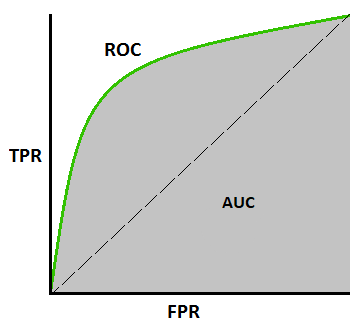
\includegraphics[scale=0.5]{chapter2/images/auc_roc.png}
		\caption[AUC - ROC Curve]{AUC - ROC Curve\textsuperscript{\cite{auc_roc}}}
    	\label{fig:auc_roc}
\end{figure} 

จากรูปที่ \ref{fig:auc_roc} เส้นโค้ง ROC สามารถหาได้ด้วยการนำค่า True positive rate (TPR) และ False positive rate (FPR) มาสร้างเป็นกราฟ โดยค่า TPR จะอยู่ในแกน y และค่า FPR จะอยู่ในแกน x ซึ่งสามารถหาค่าของ TPR และ FPR ได้ดังนี้

\begin{equation}
TPR = \frac{TP}{TP + FN}
\end{equation}
โดยที่
\begin{conditions}
TP		&		จำนวนของข้อมูลที่มีผลลัพธ์เป็นจริงและผลจากโมเดลปัญญาประดิษฐ์เป็นจริง		\\
FN		&		จำนวนของข้อมูลที่มีผลลัพธ์เป็นจริงและผลจากโมเดลปัญญาประดิษฐ์เป็นเท็จ
\end{conditions}

\begin{equation}
FPR = \frac{FP}{FP + FN}
\end{equation}
โดยที่
\begin{conditions}
FP		&		จำนวนของข้อมูลที่มีผลลัพธ์เป็นเท็จและผลจากโมเดลปัญญาประดิษฐ์เป็นจริง		\\
FN		&		จำนวนของข้อมูลที่มีผลลัพธ์เป็นจริงและผลจากโมเดลปัญญาประดิษฐ์เป็นเท็จ
\end{conditions}